% !TeX document-id = {3c9fb181-ef8d-46f4-a369-f483876e4c37}
% !TeX TXS-program:compile = txs:///pdflatex/[--shell-escape]


\documentclass[fleqn,11pt,aspectratio=169]{beamer}
\usepackage{tubslogo}
\usepackage{amsmath}
\usepackage{amsfonts}
\usepackage{amssymb}
\usepackage{graphicx}
\usepackage{qrcode}
\usepackage{geometry}
\usepackage{tikz}
\usepackage{amsthm}
\usepackage{float}
\usepackage{cleveref}
\usepackage{acronym}
\usepackage{algpseudocode}

\usepackage{fancyvrb}
\usepackage{fvextra}
\usepackage[normalem]{ulem}
\usepackage{enumerate}

\usepackage[overload]{textcase}
\usepackage{minitoc}        
%\usepackage{etoc}        
\usepackage{printlen}
\usepackage{url}  
\usepackage{tabularx}  
\usepackage{soul}
\usepackage{siunitx}
\usepackage{eqparbox}
\sisetup{
	per-mode=symbol,
}
\usepackage[utf8]{inputenc}
\usepackage[
	backend=biber,
	style=numeric,
]{biblatex}

\usepackage[rgb,dvipsnames]{xcolor}

\selectcolormodel{natural}
\usepackage{ninecolors}
\selectcolormodel{rgb}
\usepackage{tabularray}
\usepackage{minted}
\usemintedstyle{emacs,tabsize=2,linenos,xleftmargin=10pt,highlightcolor=cyan}

\usepackage[export]{adjustbox}% http://ctan.org/pkg/adjustbox

\usepackage[append]{beamersubframe}
\usepackage[american]{babel}
\usepackage{graphicx}
\setbeamerfont{normal text}{size=12pt}

\date{July 02, 2026}
\usetheme[%
  %nexus,%        Nexus Fonts benutzen
  %lnum,%         Versalziffern verwenden
  %cmyk,%<rgbprint>,          Auswahl des Farbmodells
  blue,%<orange/green/violet> Auswahl des Sekundärfarbklangs
  dark,%<light,medium>        Auswahl der Helligkeit
  %colorhead,%    Farbig hinterlegte Kopfleiste
  %colorfoot,%    Farbig hinterlegt Fußleiste auf Titelseite
  colorblocks,%   Blöcke Farbig hinterlegen
  %nopagenum,%    Keine Seitennumer in Fußzeile
  %nodate,%       Kein Datum in Fußleiste
  tocinheader,%   Inhaltsverzeichnis in Kopfleiste
  %tinytocinheader,% kleines Kopfleisten-Inhaltsverzeichnis
  %widetoc,%      breites Kopfleisten-Inhaltsverzeichnis
  %narrowtoc,%    schmales Kopfleisten-Inhaltsverzeichnis
  %nosubsectionsinheader,%  Keine subsections im Kopfleisten-Inhaltsverzeichnis
  %nologoinfoot,% Kein Logo im Fußbereich darstellen
  ]{tubs}
% Titelseite
%\title{towards TPU: A Survey into Accelerators for Cloud AI}
\title{Algorithm Engineering 2026: Sheet 04 \& 05}
\author{Rouven Kniep}

%titlepage font and background
\setbeamercolor{titlebarfirst}{parent=titlepage, bg=titlepage.bg!0}

% Edit the TUBS template to move the tubslogo into place for the title
\let\tubslogoAbsOld\tubslogoAbs
\renewcommand{\tubslogoAbs}[1]{\raisebox{-2.3mm}{\tubslogoAbsOld{#1}}}

% Quoteblock 
\newcommand{\quotebox}[1]{\begin{center}\fcolorbox{white}{blue!15!gray!15}{\begin{minipage}{0.9\linewidth}\vspace{10pt}\center\begin{minipage}{0.8\linewidth}{\space\Huge``}{#1}{\hspace{1.5em}\break\null\Huge\hfill''}\end{minipage}\smallbreak\end{minipage}}\end{center}}



\begin{document}

\part{main}
\begin{frame}[plain]
	\titlepage
\end{frame}	


\section{HW04 Pt.1}

\begin{frame}{HW04 (Crate Booking) Pt1: Setting}
\begin{columns}[T]
	\column{0.45\textwidth}
	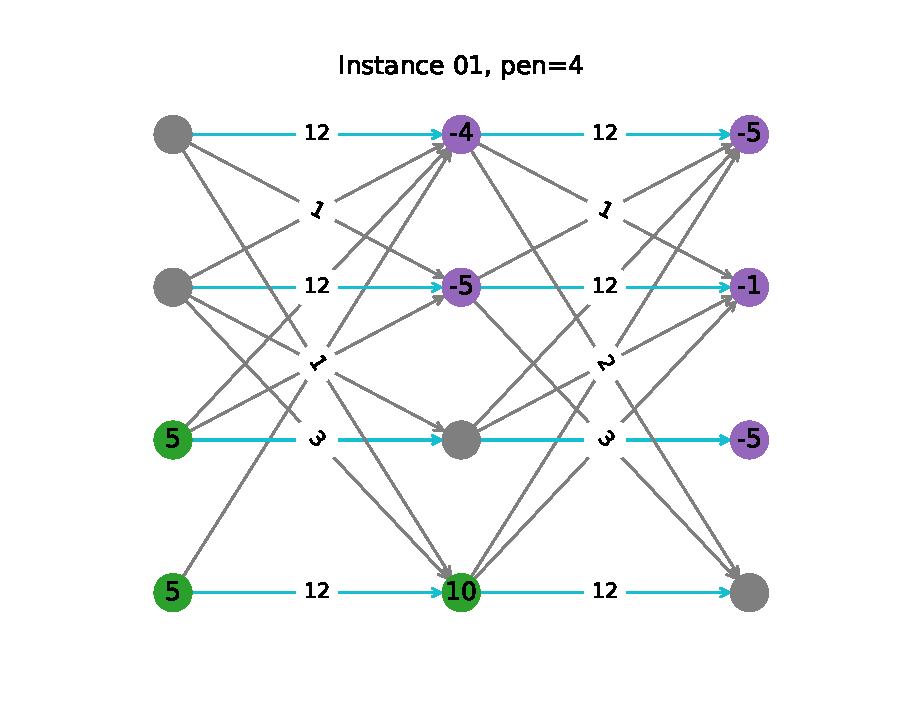
\includegraphics[keepaspectratio, scale=0.5]{instance_01_free.pdf}
	\column{0.5\textwidth}
	\begin{itemize}
		\item \textbf{Depots} (rows)
		\item \textbf{Days} (columns)
		\item \textbf{Node}: days $\times$ depots
		\item \textbf{Balance}: surplus / demand at some nodes
		\item \textbf{free Arcs}: node to node with capacity (1st element)
		\item \textbf{Trucks}: not available! free flow only
		\item \textbf{Unmet Penalty}: penalty for each crate of unmet demand
	\end{itemize}
\end{columns}
\end{frame}

\begin{frame}{HW04 (Crate Booking) Pt1: Solution}
	\begin{columns}[T]
		\column{0.45\textwidth}
		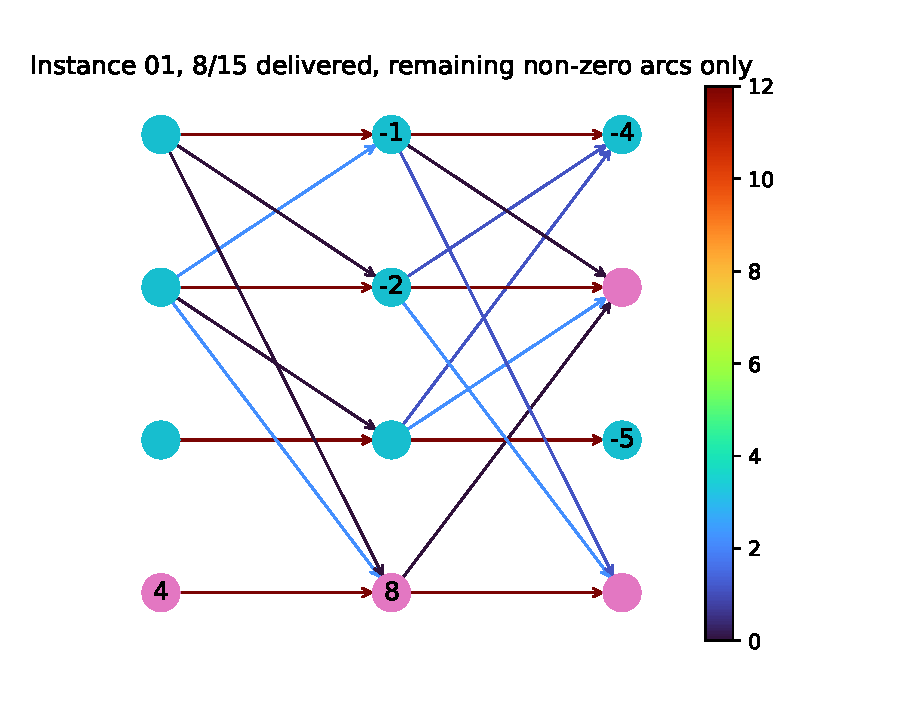
\includegraphics[keepaspectratio, scale=0.5]{instance_01_free_sol.pdf}
		\column{0.5\textwidth}
		\begin{itemize}
			\item omitted SuperSource \& SuperSink
			\item \textbf{Max Flow}: (one) allocation (edge$\rightarrow$flow) with maximum total flow
			\item \textbf{Min Cut}: (one) 2-partition of nodes (before the cut, after the cut)
			\item all forward edges across cut: fully utilized $\implies$ more cap/trucks \textbf{might} help
			\item edges within a partition (or backwards across cut): more capacity \textbf{cannot} help
			\item \textbf{Planners}: book trucks across cut towards underutilized edges, insert + reevaluate
		\end{itemize}
	\end{columns}
\end{frame}

\section{HW04 Pt.2}


\begin{frame}{HW04 (Crate Booking) Pt2: Setting}
	\begin{columns}[T]
		\column{0.45\textwidth}
		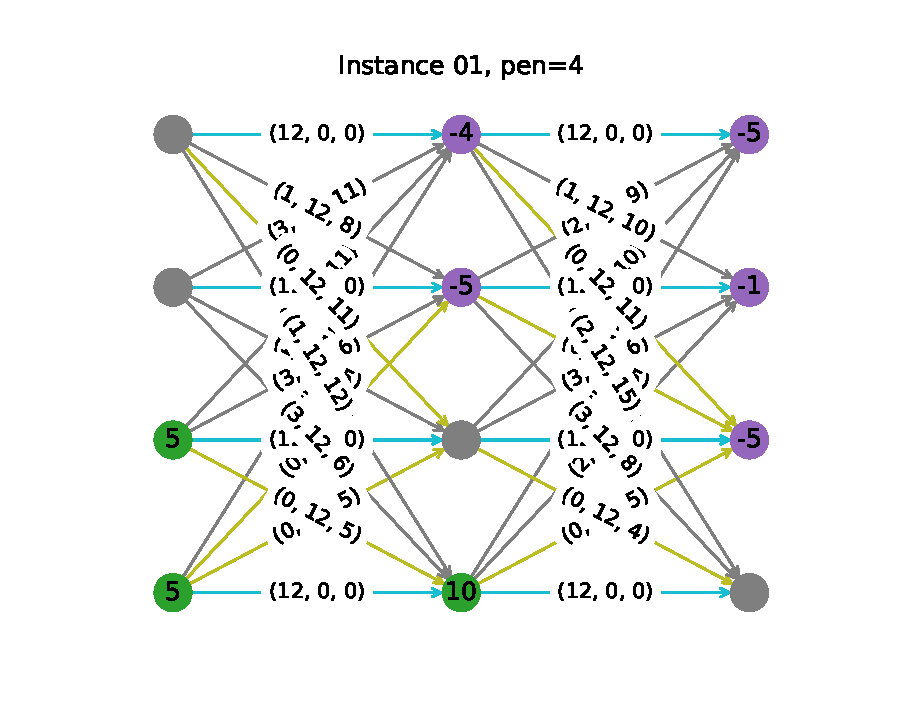
\includegraphics[keepaspectratio, scale=0.5]{instance_01.pdf}
		\column{0.5\textwidth}
		\begin{itemize}
			\item \textbf{Depots} (rows)
			\item \textbf{Days} (columns)
			\item \textbf{Node}: days $\times$ depots
			\item \textbf{Balance}: surplus / demand at some nodes
			\item \textbf{free Arcs}: node to node with capacity (1st element)
			\item \textbf{Trucks}: node to node,\\capacity (2nd) \& cost (3rd) per truck
			\item \textbf{Unmet Penalty}: penalty for each crate of unmet demand
		\end{itemize}
	\end{columns}
\end{frame}

\begin{frame}{Crate Booking Model}
	\begin{columns}[T]
		\column{0.45\textwidth}
		Idea: use graph as data structure
		\begin{itemize}
			\item can store any data in nodes / edges
			\item available query-operations
			\item native to our problem
			\item partially implemented from Pt.1
		\end{itemize}
		\column{0.45\textwidth}	
		problem native:
		\begin{itemize}
			\item for each edge...
			\begin{itemize}
				\item flow: decision var
				\item booked trucks: decision var
				\item capacity: constraint
				\item obj+= truck costs
			\end{itemize}
			\item for each node...
			\begin{itemize}
				\item flow conservation: constraint
				\item obj+= unmet demand penalty
			\end{itemize}
			\item minimize objective penalty
		\end{itemize}
	\end{columns}
\end{frame}



\begin{frame}[fragile,t]{Edge Modeling}
\begin{minted}[highlightlines={6,7,8}]{python}
def _model_edge_flow(self):    # model edge flow + trucks
	for src, dst, data in self.g.edges(data=True):
		data["flow_var"] = self.var(lb=0, name=f"flow_{src}_{dst}")
		if data.get("truck_cap", 0) != 0:
			data["truck_var"] = self.intvar(lb=0, name=f"trucks_{src}_{dst}")
			self.model.add_linear_constraint(
				data["flow_var"] <= data.get("capacity", 0) 
				+ data["truck_cap"] * data["truck_var"])
			self.objective += data["truck_var"] * data.get["truck_cost"]	
		else:
			self.model.add_linear_constraint(
				data["flow_var"] <= data.get("capacity", 0))
\end{minted}
\end{frame}

\begin{frame}[fragile,t]{Node Modeling[1]}	
	\begin{minted}[highlightlines={4,6}]{python}    
def _model_node_flow(self):
	for node, ndata in self.g.nodes(data=True):
		incoming = [var for src, dst, var 
			in self.g.in_edges(nbunch=node, data="flow_var")]
		outgoing = [var for src, dst, var 
			in self.g.out_edges(nbunch=node, data="flow_var")]
		delta = ndata.get("net", 0)
		flow = sum(incoming) - sum(outgoing)
	\end{minted}
	\vspace{20pt}
	"problem native" data structure: query operations!
\end{frame}
\begin{frame}[fragile,t]{Node Modeling[2]}	
	\begin{minted}[highlightlines={3,7,9}]{python}
		# node flow equality: in - out + unmet_pen + delta >= 0    
		if delta > 0:
			c = flow + delta >= 0 c # allow not picking up
		elif delta < 0:
			ump = self.var(lb=0, ub=-delta, name=f"unmet_pen_{node}")
			self.objective += ump * self.instance.unmet_penalty
			c = flow + ump + delta == 0
		else:
			c = flow == 0
		self.model.add_linear_constraint(c, name=f"node_flow_{node}")		
	\end{minted}
\end{frame}


\begin{frame}{HW04 (Crate Booking) Pt2: Example Solution}
	\begin{center}
		\colorbox{black}{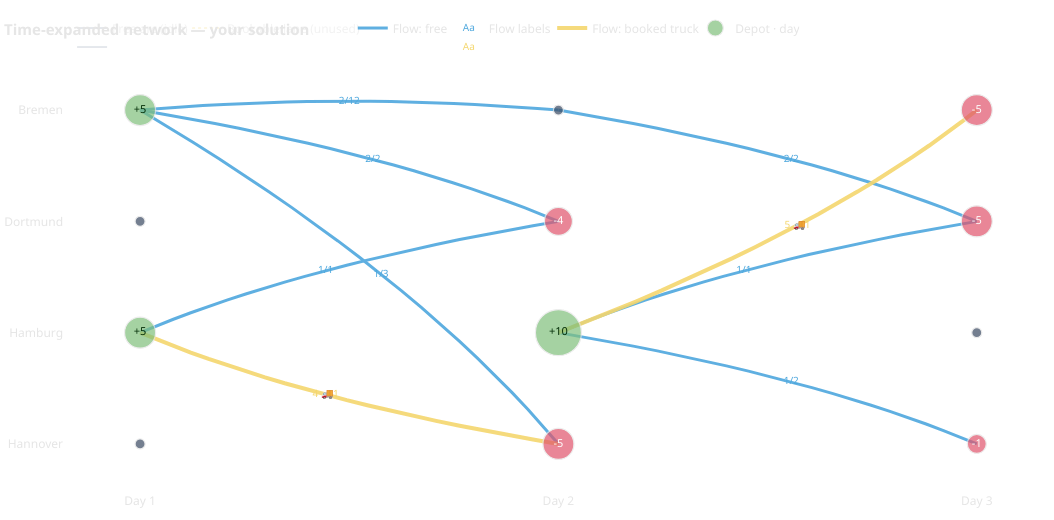
\includegraphics[keepaspectratio, height=0.8\textheight]{instance_01_sol.png}} 
	\end{center}
\end{frame}

\begin{frame}{HW04 (Crate Booking) Pt2: Linear Programming Relaxation}
	\begin{itemize}
		\item "solve LP relaxation": replace \textbf{all} integer variables with continuous
		\item "explain why it is a \textit{strict} lower bound"
		\begin{itemize}
			\item \texttt{relaxation} $\subseteq$ \texttt{integer model} $\land$ \texttt{minimization} $\implies$ \texttt{lower bound}
			\item "\textit{strict}": doesn't say anything: objective can be the same!
		\end{itemize}
		\item "Why a MIP?"
		\begin{itemize}
			\item partial usage of a truck $\implies$ full payment: \texttt{flow} $\leq$ \texttt{capacity} $+$ \texttt{truck\_cap} $*$ \texttt{truck\_var}
			\item therefore \texttt{truck\_var} must be non-continuous integer - rest can be continuous and linear
			\item LP (P-time) $\rightarrow$ MIP (NP-hard)
		\end{itemize}
	\end{itemize}
\end{frame}

\section{HW05 Ex1}

\begin{frame}{HW05 Ex1 Setting: $n$ Queens}
	\begin{columns}
		\column{0.45\textwidth}
		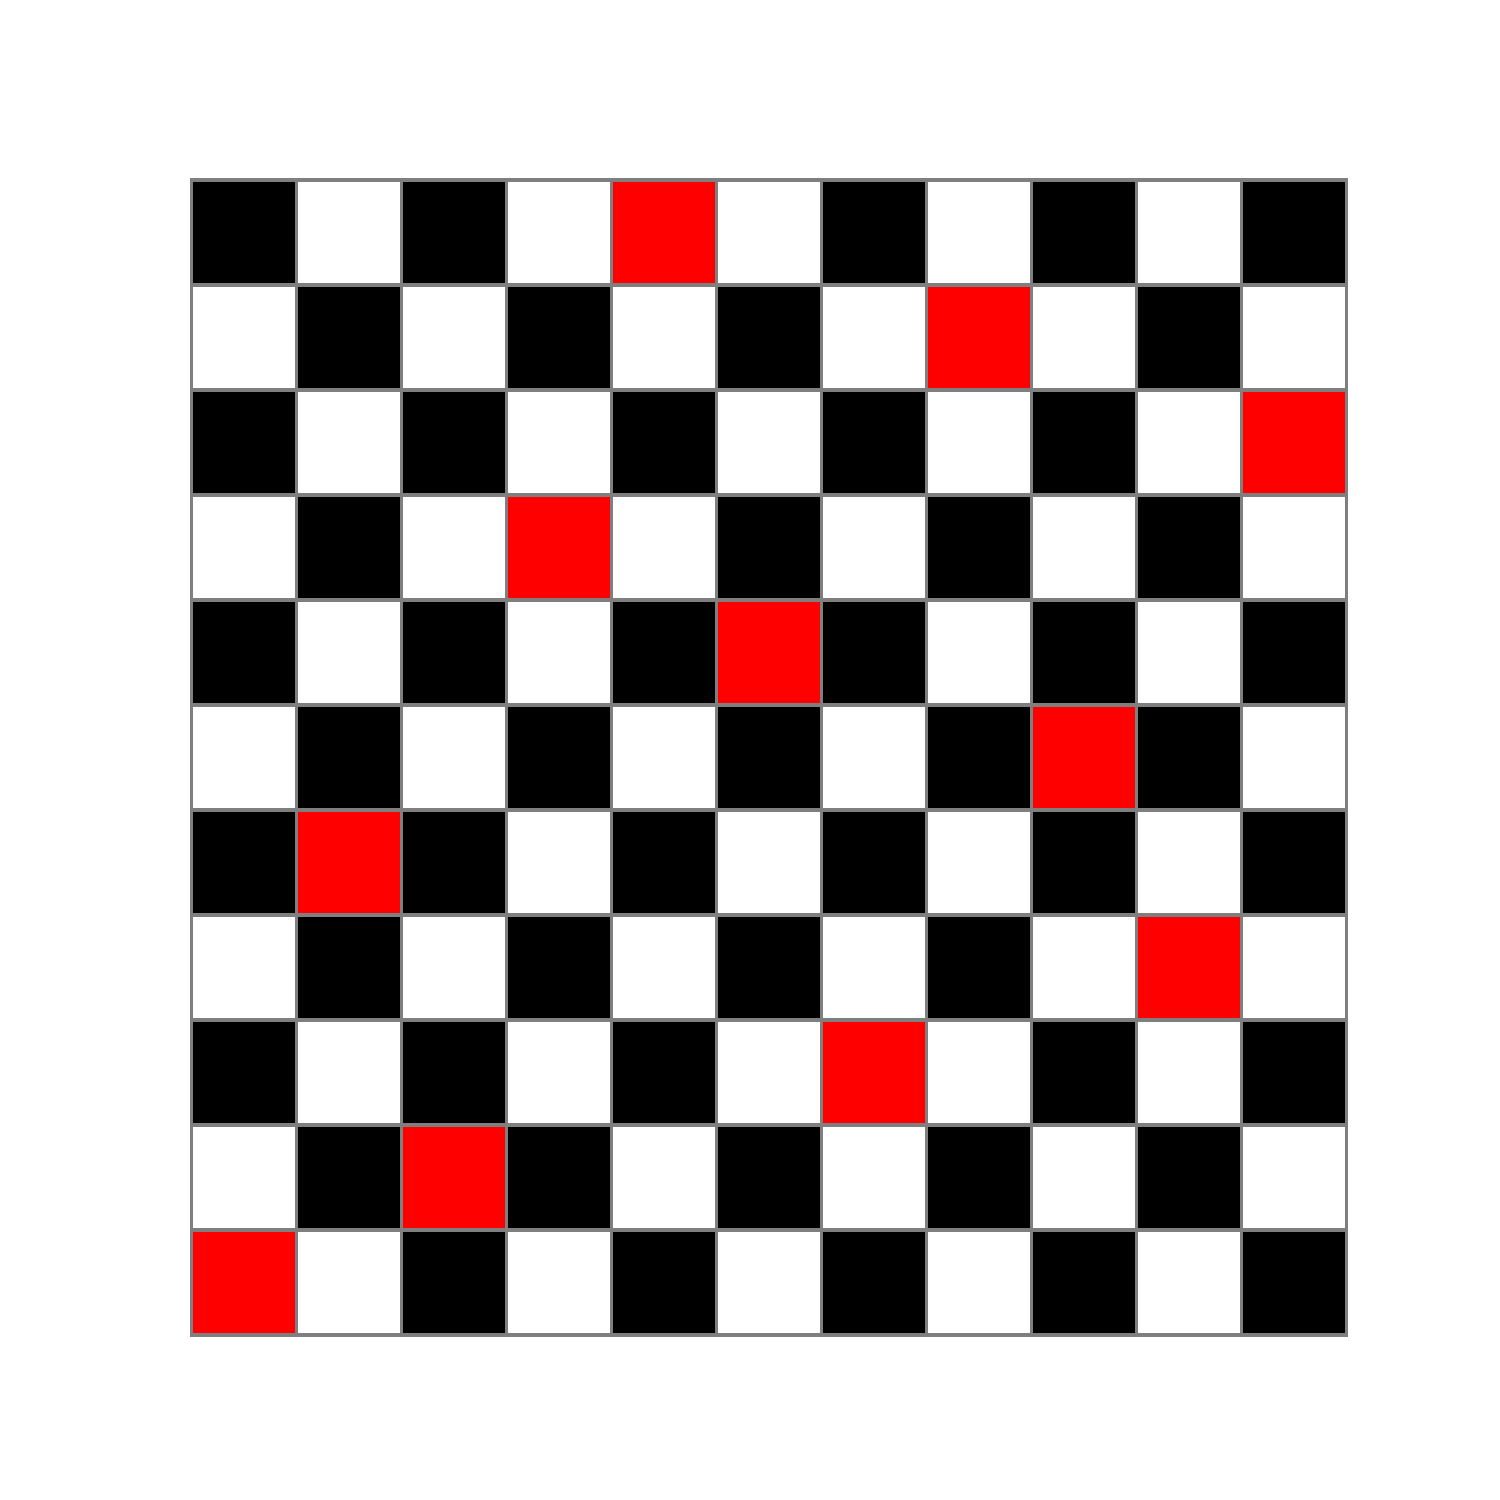
\includegraphics[width=\columnwidth, keepaspectratio]{queens_11.pdf}
		\column{0.45\textwidth}	
		\begin{itemize}
			\item $n*n$ chess grid
			\item $n$ queens
			\item position queens on the chess field
			\item no queen can see another
		\end{itemize}
	\end{columns}
\end{frame}

\begin{frame}{$n$ Queens: Constraints (visualized)}
\begin{columns}
	\column{0.45\textwidth}
	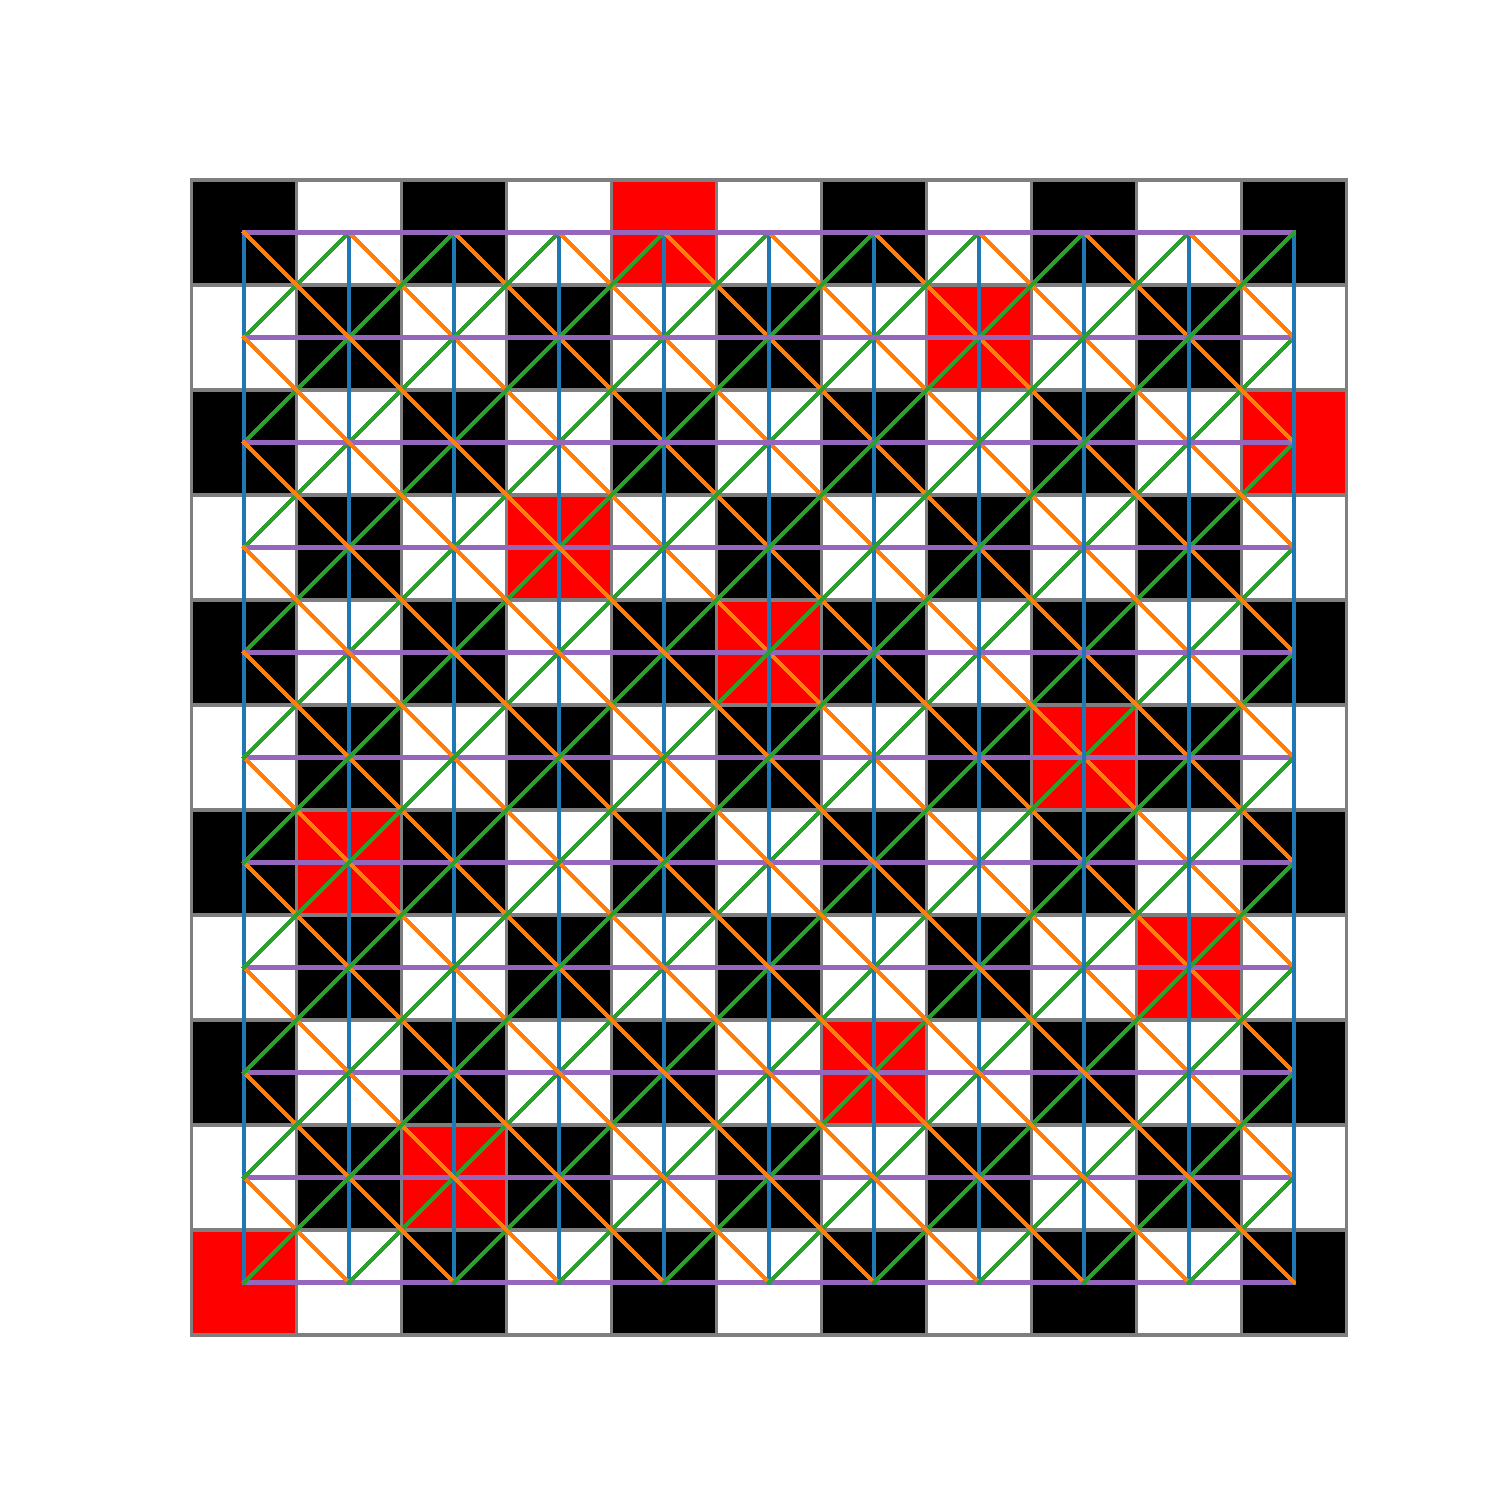
\includegraphics[width=\columnwidth, keepaspectratio]{queens_11_constraints.pdf}
	\column{0.45\textwidth}	
	Constraints:
	\begin{itemize}
		\item \textcolor[HTML]{1f77b4}{exactly one per column}
		\item \textcolor[HTML]{9467bd}{exactly one per row}
		\item \textcolor[HTML]{2ca02c}{at most one per "positive" diagonal}
		\item \textcolor[HTML]{ff7f0e}{at most one per "negative" diagonal}
	\end{itemize}
\end{columns}
\end{frame}

\begin{frame}{$n$ Queens: Constraints (formalized)}
\begin{tblr}{colspec={c|c|r l},hlines}
	\SetCell[r=3]{} {columns\\(rows similar)} & cardinality &  $\sum_{y=0}^{n-1} b_{xy} = 1$ & $\forall x\in [0,n-1]$ \\
		& \SetCell[r=2]{} SAT (CNF) & $\lor_{y=0}^{n-1}b_{xy}$ & $ \forall x\in [0,n-1]$ \\
								&& $\neg b_{xy} \lor \neg b_{iy}$ & $\forall i,x,y \in [0,n-1]^3 \mid i \neq x$ \\
	\SetCell[r=2]{} {positive diagonal\\(negative similar)} & cardinality & $(\sum b_{xy} \mid x-y = k) \leq 1$ & $\forall k\in [-n+2;n-2]$ \\
								& SAT (CNF)& $\neg b_{ij} \lor \neg b_{xy} $ & {$\forall x,y,i,j \in [0,n-1]^4$\\$\mid i+j=x+y \land i \neq x$} \\
\end{tblr}
\end{frame}


\begin{frame}[fragile,t]{$n$ Queens: Constraints implementation}	
	\begin{minted}[]{python}
self.cnf.extend(list(self.iter_row_lits(row)) for row in range(self.n))
self.cnf.extend(list(self.iter_col_lits(col)) for col in range(self.n))
for row in range(self.n):
	self.cnf.extend((-l1, -l2) for l1, l2 in self.iter_row_combinations(row))
for col in range(self.n):
	self.cnf.extend((-l1, -l2) for l1, l2 in self.iter_col_combinations(col))
for k in range(2 * self.n):  # "sum" diagonal
	self.cnf.extend((-l1, -l2) 
		for l1, l2 in self.iter_neg_diag_combinations(k))
for k in range(-self.n + 1, self.n):  # "difference" diagonal
	self.cnf.extend((-l1, -l2) 
		for l1, l2 in self.iter_pos_diag_combinations(k))
	\end{minted}
\end{frame}

		
\begin{frame}{$n$ Queens: Symmetry Breaking}
	\begin{columns}
		\column{0.45\textwidth}
		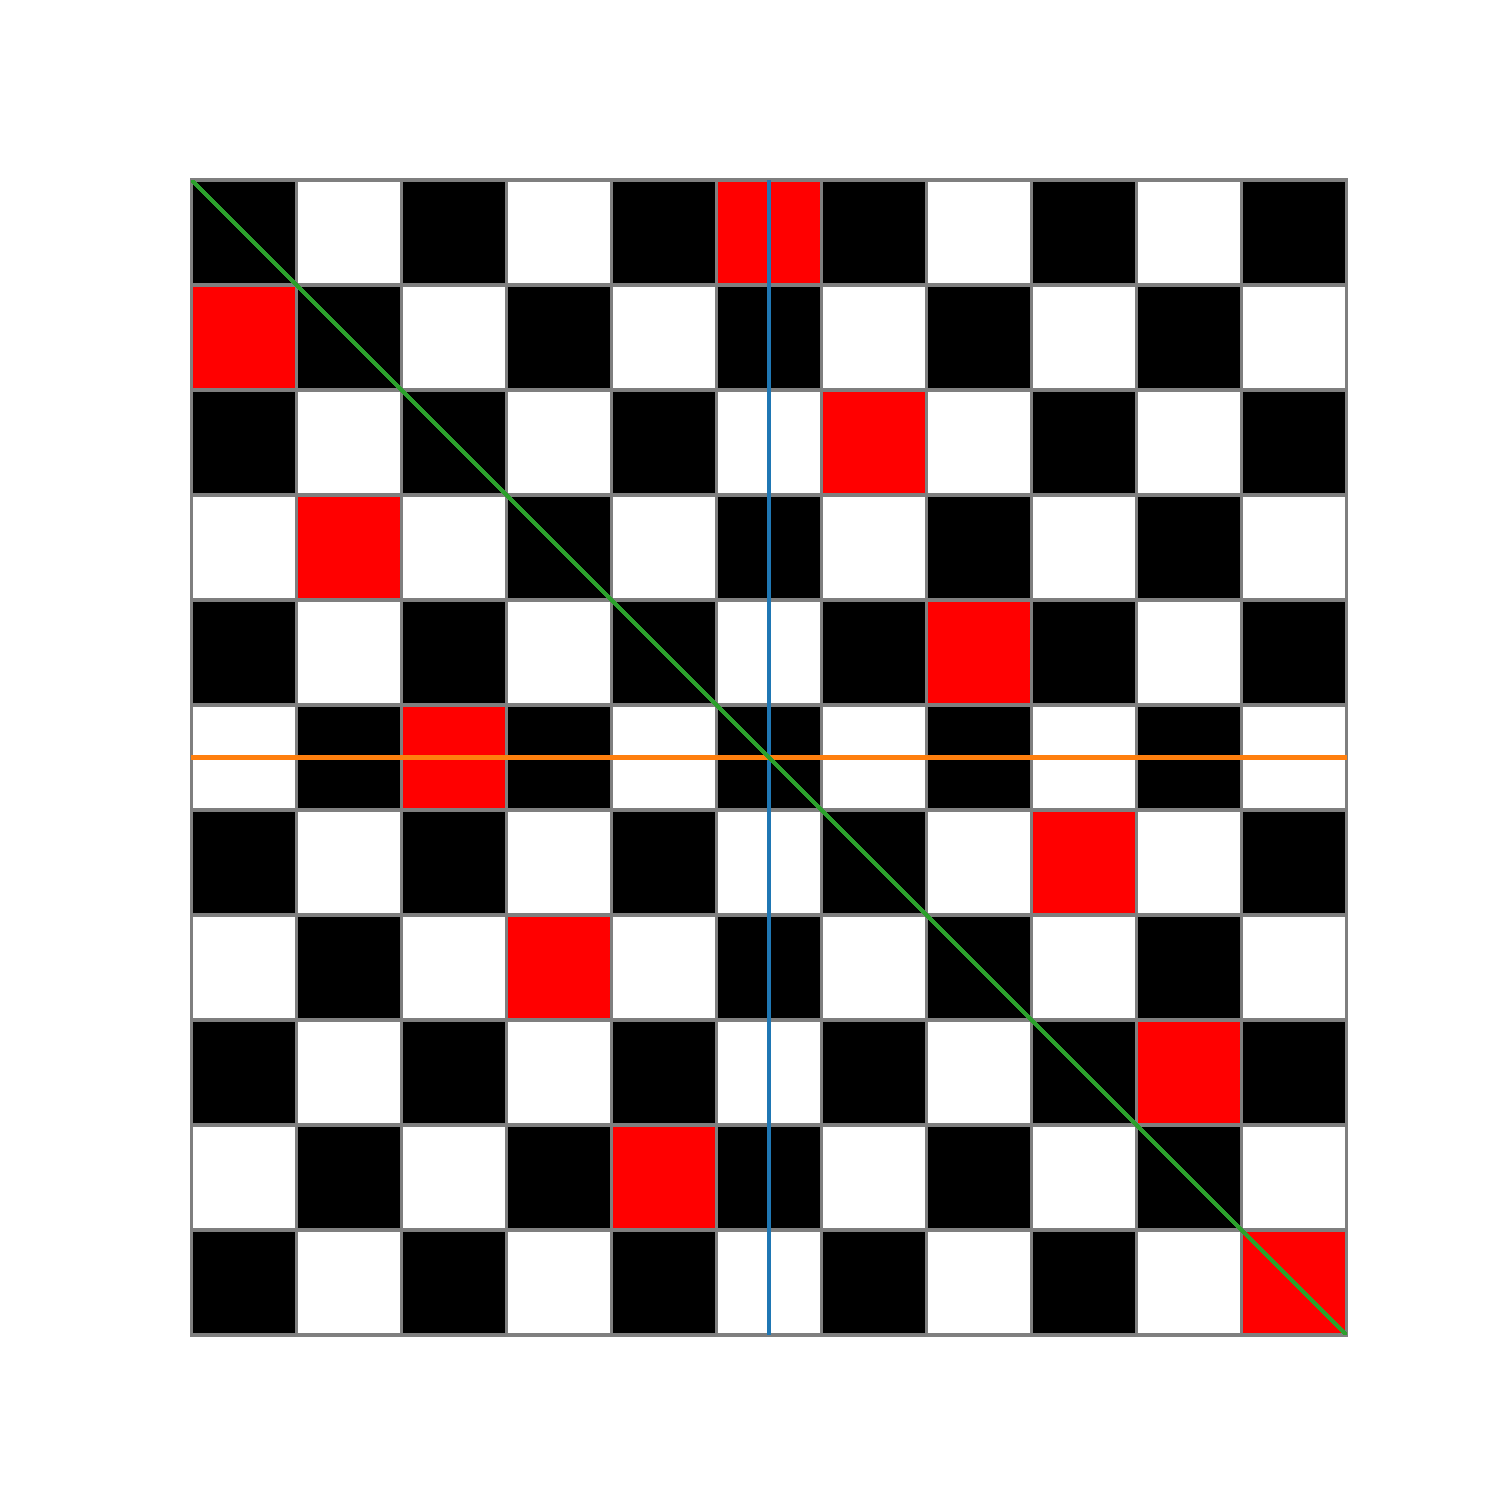
\includegraphics[width=\columnwidth, keepaspectratio]{queens_11_symmetry.pdf}
		\column{0.45\textwidth}	
		Symmetries:
		\begin{itemize}
			\item \textcolor[HTML]{1f77b4}{horizontal}: row 0 queen must be in right half
			\item \textcolor[HTML]{ff7f0e}{vertical}: row 0 queen must be right of row n-1 queen
			\item \textcolor[HTML]{2ca02c}{diagonal}: row 0 queen column number must be equal or lower than column 0 queen row number 
			\item ... more possible (positive diagonal)
		\end{itemize}
	\end{columns}
\end{frame}		

\begin{frame}[fragile,t]{$n$ Queens: Symmetry Breaking implementation}
	\begin{minted}[]{python}
self.cnf.append([self.get_lit(0, col) for col in range(ceil(self.n / 2))])
		
for topcol in range(1, ceil(self.n / 2)):
	toplit = self.get_lit(0, topcol)
	# vertical
	self.cnf.extend([-toplit, -self.get_lit(self.n - 1, bottomcol)]
		for bottomcol in range(topcol))
		
	# negative diagonal
	for col in range(1, ceil(self.n / 2)):
		toplit = self.get_lit(0, col)
		self.cnf.extend([-toplit, -self.get_lit(row, 0)] 
			for row in range(col))
	\end{minted}
\end{frame}

\begin{frame}[fragile,t]{$n$ Queens: CP-SAT cardinality}
	\begin{minted}[]{python}
# rows/cols: exactly one        
for row in range(self.n):
	self.model.add_exactly_one(self.iter_row_lits(row))
for col in range(self.n):
	self.model.add_exactly_one(self.iter_col_lits(col))

# diagonals: at most one		
for row in range(0, self.n):
	self.model.add_at_most_one(self.iter_diagonal_lits(row, 0, positive=True))
	self.model.add_at_most_one(self.iter_diagonal_lits(row, 0, positive=False))
for col in range(0, self.n):
	self.model.add_at_most_one(self.iter_diagonal_lits(0, col, positive=True))
	self.model.add_at_most_one(self.iter_diagonal_lits(self.n - 1, col, positive=False))
	\end{minted}
\end{frame}

\begin{frame}[fragile,t]{$n$ Queens: CP-SAT integers (official version!)}
	\begin{minted}[]{python}        
# one per row -> var
self.vars = [self.model.new_int_var(0, self.n - 1, name=f"q{row}") 
	for row in range(self.n)

self.model.add_all_different(self.vars)	# one per column

# positive diagonals
self.model.add_all_different([var + row 
	for row, var in enumerate(self.vars)])

# negative diagonals
self.model.add_all_different([var - row 
	for row, var in enumerate(self.vars)])
	\end{minted}
\end{frame}


\begin{frame}{$n$ Queens: Benchmarks}
	Limits: CNF-SAT 350 (memory, 160s), CP-SAT int 350 (time), CP-SAT card 1500 (memory, 60s)
	\begin{columns}[T]
		\column{0.48\textwidth}
		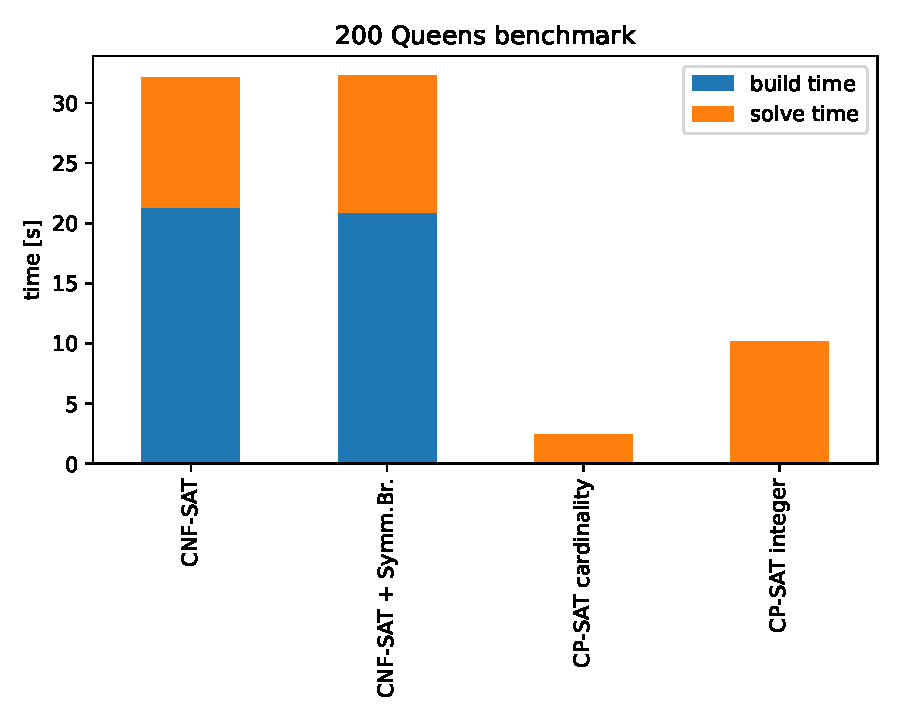
\includegraphics[width=\columnwidth, keepaspectratio]{queens200bench.pdf}
		\column{0.48\textwidth}
		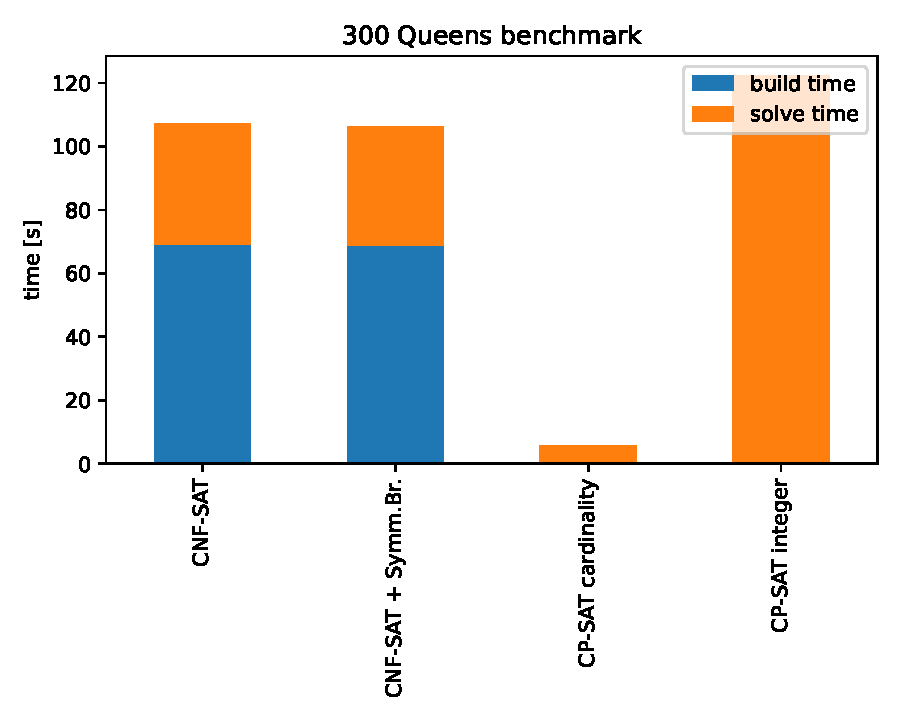
\includegraphics[width=\columnwidth, keepaspectratio]{queens300bench.pdf}
	\end{columns}
\end{frame}

\section{HW05 Ex2}

\begin{frame}{HW05 Ex2a: CNF Bounded Variable Elimination Correctness}
	"$\implies$" ($\varphi$ SAT $\implies \varphi'$ SAT):
	\begin{itemize}
		\item Clauses in $\varphi'$ that are in $\varphi$ are naturally satisfied.
		\item All other clauses in $\varphi'$ are of form $A \lor B$ as a result of resolving $(x\lor A) \land (\neg x \lor B) \in \varphi$.
		\item If $x \in S$: as $S\models \neg x \lor B$, then $S\models B$, which implies $S\models A \lor B$ and therefore $S \models \varphi'$
		\item If $\neg x \in S$: as $S\models x \lor A$, then $S\models A$, which implies $S\models A \lor B$ and therefore $S \models \varphi'$ 
	\end{itemize} 
	"$\impliedby$" ($S'$ SAT $\implies S'$ SAT):
	\begin{itemize}
		\item let $S_+ = S'\cup {x}$ and $S_- = S'\cup {\neg x}$
		\item W.l.o.g. let $S_+ \not\models \varphi$: reason must be $\neg x\lor B = \bot$ that was removed and is not satisfied by $x=\top$
		\item $S' \models A \lor B$ forall $A$ as $S' \not\models B$, therefore $S_-\models \varphi$:
		\item as $S' \models A \implies S'\models x\lor A$, and $S_-\models \neg x \lor B$ naturally.
	\end{itemize} 
\end{frame}

\begin{frame}{HW05 Ex2b: CNF Vivification}
	let $C = l_1 \lor ... \lor l_k$, with propagation $P = \neg l_1 \land ... \land \neg l_j$
	\begin{enumerate}
		\item $P \implies l_i \mid k \geq i \ge j$: $C$ can be removed, as $(P\land l_i) \models C$. \\ 
				in practice: not necessarily effective!
		\item $P \implies \neg l_i \mid k \geq i \ge j$: $C$ can be strengthened into $C'$ by removing $l_i$.\\
		That would change satisfiability of $S$, iff $c_i = \top \land \forall 1\leq l \leq k \land l\neq i: c_l = \bot$, but $\neg l_1 \land ... \land \neg \l_k \implies \neg c_i$, which contradicts.
		\item $\neg l_1 \land ... \land \neg l_j$ causes a conflict: we learn $N = l_1 \lor ... \lor l_j \subset C$ and can remove $C$.
	\end{enumerate}
\end{frame}

\begin{frame}{HW05 Ex2c: CNF Blocked Clause Elimination}
	let $C = l \lor a_1 \lor ... \lor a_k \in \varphi$. 
	
	$C$ is  \textit{blocked on} $l$ if $\forall D \mid \neg l \in D: C \diamond_l D \implies \top$ and can then be removed
	
	"$\impliedby$" ($\varphi$ SAT $\implies \varphi'$ SAT): trivial, as $\forall P \mid P \models \varphi \implies P \models \varphi'$. 
	
	"$\implies$ ($\varphi'$ SAT $\implies \varphi$ SAT): let $S'\models \varphi'$
	\begin{itemize}
		\item If $S' \models \varphi$: done.
		\item If $S' \not\models \varphi$, then $S' \not\models C$ and therefore $\neg l \in S'$. 
		\item let $S=(S'\setminus {\neg l} \cup {l})$, then $S \models C$, but might not model a $D$. 
		\item however $\forall D: \exists a_i \mid 1\leq i \leq k: \neg a_i \in D$, which is given by above. 
		\item therefore $\forall D: S \models D$ 
	\end{itemize}
\end{frame}


\end{document}
